\documentclass[paper]{IEEEtran}
\IEEEoverridecommandlockouts
% The preceding line is only needed to identify funding in the first footnote. If that is unneeded, please comment it out.
\usepackage[english]{babel}
\usepackage[utf8x]{inputenc}
\usepackage{amsmath}
\usepackage{graphicx}
\usepackage[colorinlistoftodos]{todonotes}
\usepackage{gensymb} % this could be problem
\usepackage{float}
\usepackage{fancyref}
\usepackage{subcaption}
\usepackage{amssymb}

\usepackage{pythonhighlight}

\usepackage{xspace}

\newcommand\nd{\textsuperscript{nd}\xspace}
\newcommand\rd{\textsuperscript{rd}\xspace}
\newcommand\nth{\textsuperscript{th}\xspace} %\th is taken already


\usepackage{xcolor}
\usepackage{listings}

\usepackage{fancyhdr}

\usepackage{karnaugh-map}

\definecolor{mGreen}{rgb}{0,0.6,0} % for python
\definecolor{mGray}{rgb}{0.5,0.5,0.5}
\definecolor{mPurple}{rgb}{0.58,0,0.82}


\definecolor{mygreen}{RGB}{28,172,0} % color values Red, Green, Blue for matlab
\definecolor{mylilas}{RGB}{170,55,241}

\lstdefinestyle{CStyle}{
	commentstyle=\color{mGreen},
	keywordstyle=\color{magenta},
	numberstyle=\tiny\color{mGray},
	stringstyle=\color{mPurple},
	basicstyle=\footnotesize,
	breakatwhitespace=false,         
	breaklines=true,                 
	captionpos=b,                    
	keepspaces=true,                 
	numbers=left,                    
	numbersep=5pt,                  
	showspaces=false,                
	showstringspaces=false,
	showtabs=false,                  
	tabsize=2,
	language=C
}


\lstset{language=Matlab,%
	%basicstyle=\color{red},
	breaklines=true,%
	morekeywords={matlab2tikz},
	keywordstyle=\color{blue},%
	morekeywords=[2]{1}, keywordstyle=[2]{\color{black}},
	identifierstyle=\color{black},%
	stringstyle=\color{mylilas},
	commentstyle=\color{mygreen},%
	showstringspaces=false,%without this there will be a symbol in the places where there is a space
	numbers=left,%
	numberstyle={\tiny \color{black}},% size of the numbers
	numbersep=9pt, % this defines how far the numbers are from the text
	emph=[1]{for,end,break},emphstyle=[1]\color{red}, %some words to emphasise
	%emph=[2]{word1,word2}, emphstyle=[2]{style},    
}



\makeatletter
\renewcommand\paragraph{\@startsection{paragraph}{4}{\z@}%
	{-2.5ex\@plus -1ex \@minus -.25ex}%
	{1.25ex \@plus .25ex}%
	{\normalfont\normalsize\bfseries}}
\makeatother
\setcounter{secnumdepth}{4} % how many sectioning levels to assign numbers to
\setcounter{tocdepth}{4}    % how many sectioning levels to show in ToC



\begin{document}
	
	\title{EE314 Digital Electronics Laboratory\\
		2017-2018 Spring Term Project Final Report\\
		An FPGA Based Oscilloscope
	}
	
	
	\author{
		
		\IEEEauthorblockN{1\textsuperscript{st} Halil TEMURTAS}
		\IEEEauthorblockA{\textit{2094522} }
		\textit{halil.temurtas@metu.edu.tr}
		
		\and
		
		\IEEEauthorblockN{2\textsuperscript{nd} Erdem TUNA}
		\IEEEauthorblockA{\textit{2167419} }
		\textit{erdem.tuna@metu.edu.tr}
		
		
	}
	
	\maketitle
	
	\begin{abstract}
		
		The design of an FPGA based digital oscilloscope 
		
	\end{abstract}
	
	\begin{IEEEkeywords}
		FGPA, oscilloscope, ADC, VGA
	\end{IEEEkeywords}
	
	\section{Introduction}
	\- \indent
	In this project, it is intended to realize a digital oscilloscope by using an FPGA. The FGPA will receive an analog signal, digitize it through an ADC; then will calculate the required parameters. Lastly data and input signal will be displayed on a VGA screen. The overall diagram is shown in \textit{Figure~\ref{fig:overall_diagram}}. The implementation logics and algorithms are discussed in respective sections.
	
	\begin{figure}[h!]
		\setlength{\unitlength}{\textwidth}
		\center 
		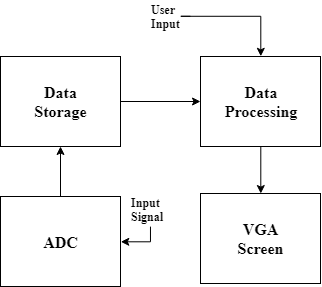
\includegraphics[width=0.47\textwidth]{overall_diagram}
		\caption{\label{fig:overall_diagram}The Block Diagram of the Project}
	\end{figure}
	
	
	\section{ALTERA DE1-SoC}
	\- \indent
	In this project, we have used ALTERA DE1$\_$SoC Development Kit for main unit and a VGA Monitor as a screen for the oscilloscope. In this part, our aim is to introduce the FPGA used in the project. The overall look of the device can be seen at \textit{Figure~\ref{fig:FPGA}}, as can be seen from the figure, the Development Kit consists of multiple parts aside from FPGA. In this project, GPIO Pins, seven segment display, push buttons, switches and VGA output of DE1-SoC was used.  
	
	\begin{figure}[H]
		\setlength{\unitlength}{\textwidth}
		\center 
		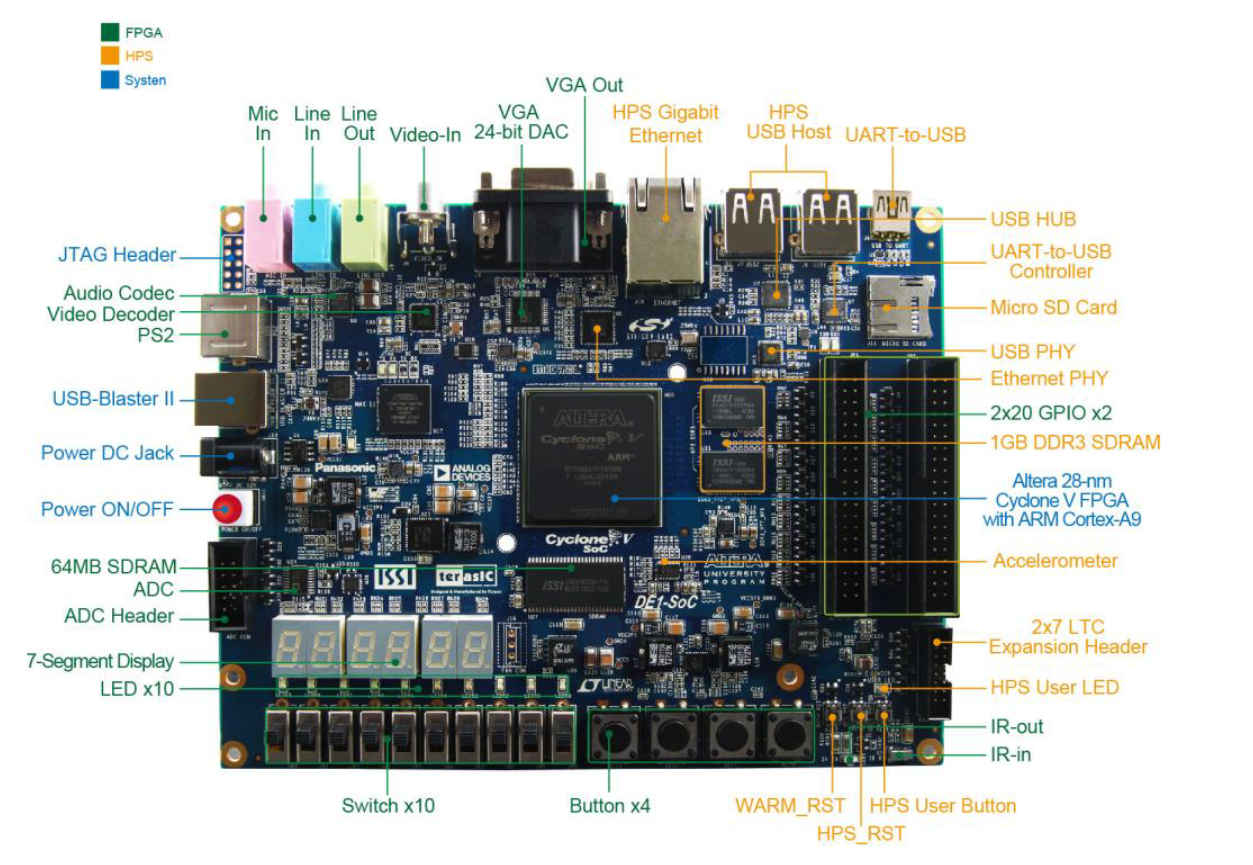
\includegraphics[width=0.47\textwidth]{FPGA}
		\caption{\label{fig:FPGA}ALTERA DE1$\_$SoC Development Kit}
	\end{figure}
	
	GPIO pins, also known as general-purpose input/output pins, were used for getting the analog input that is desired to be monitored through oscilloscope. As can be seen from the \textit{Figure~\ref{fig:GPIO}}, the basic circuitry for this pins includes Schottky diodes for protection, and a resistor.
	
	\begin{figure}[H]
		\setlength{\unitlength}{\textwidth}
		\center 
		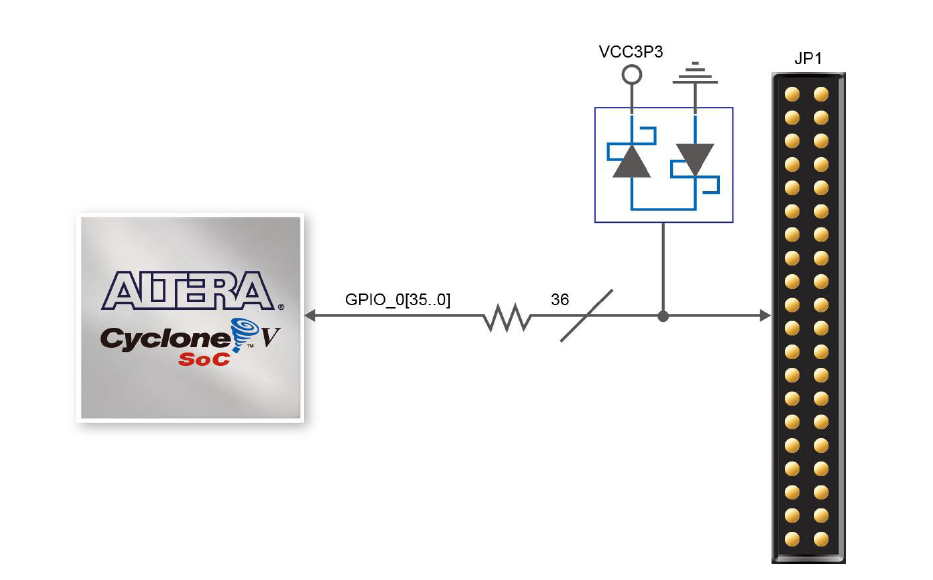
\includegraphics[width=0.47\textwidth]{GPIOpins}
		\caption{\label{fig:GPIO}GPIO Pins}
	\end{figure}
	
	Seven segment display was used for testing the output values of computation value without using external monitor that we had some difficulties to find. As can be seen from the \textit{Figure~\ref{fig:SSD}}, every led on the seven segment is connected through a resistor to the FPGA.
	
	
	\begin{figure}[H]
		\setlength{\unitlength}{\textwidth}
		\center 
		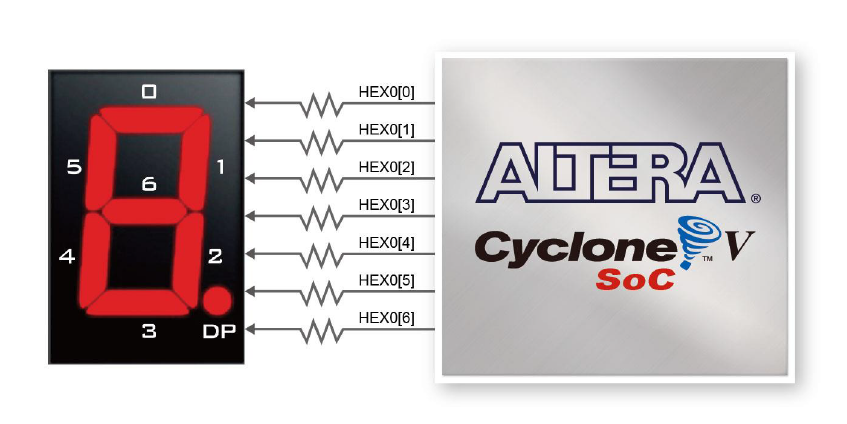
\includegraphics[width=0.47\textwidth]{SSD}
		\caption{\label{fig:SSD} Seven Segment Display}
	\end{figure}
	
	Finally, the switch buttons were used as a mode buttons of the oscilloscope and push buttons were used as a division changer for the oscilloscope. The connections to FPGA can be seen at \textit{Figure~\ref{fig:pushbuttons}} and \textit{Figure~\ref{fig:switchbuttons}}. Finally the VGA connection used will be explained later in the report. 
	
	\begin{figure}[h!]
		\setlength{\unitlength}{\textwidth}
		\center 
		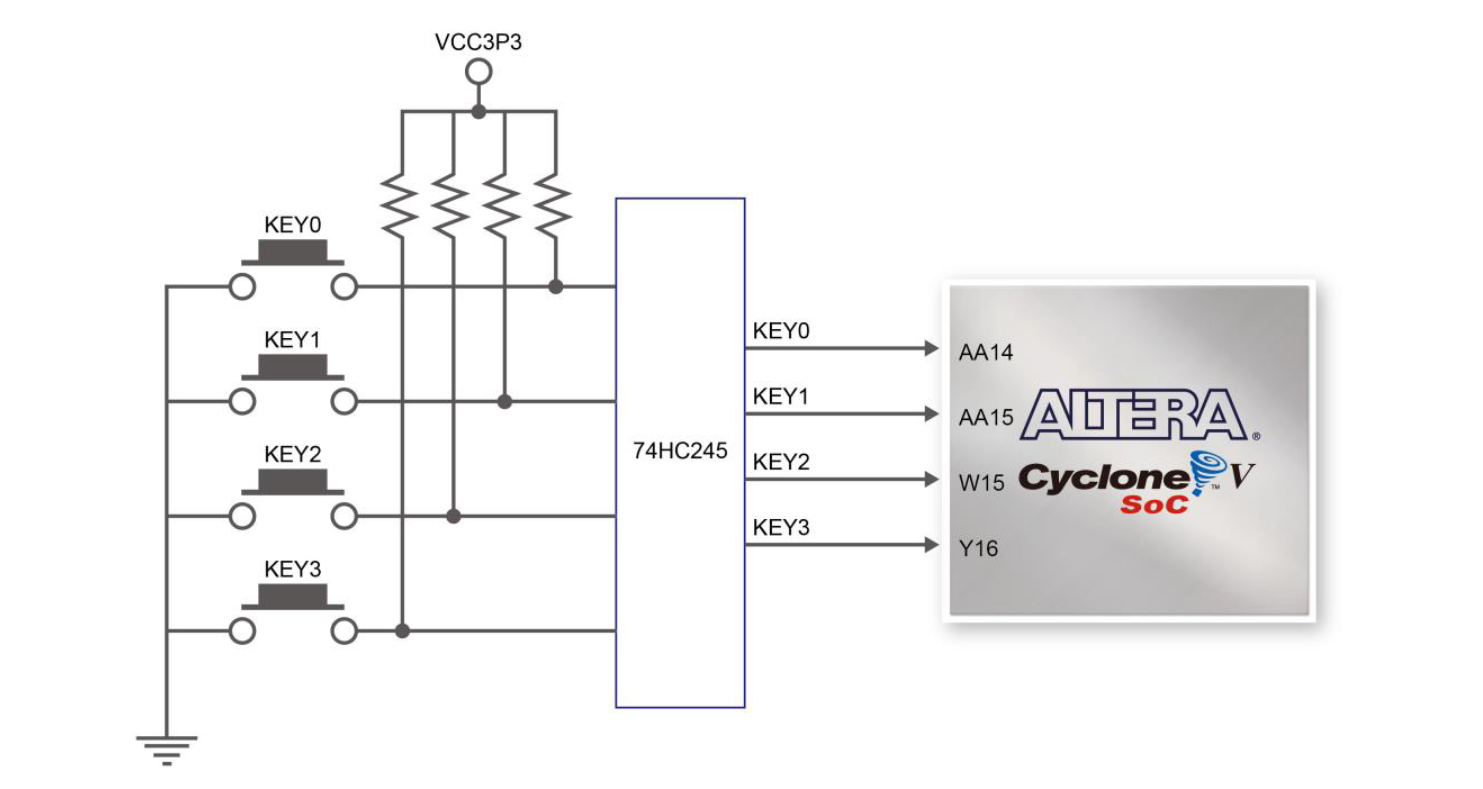
\includegraphics[width=0.47\textwidth]{pushbuttons}
		\caption{\label{fig:pushbuttons} Push Buttons}
	\end{figure}
	
	
	\begin{figure}[h!]
		\setlength{\unitlength}{\textwidth}
		\center 
		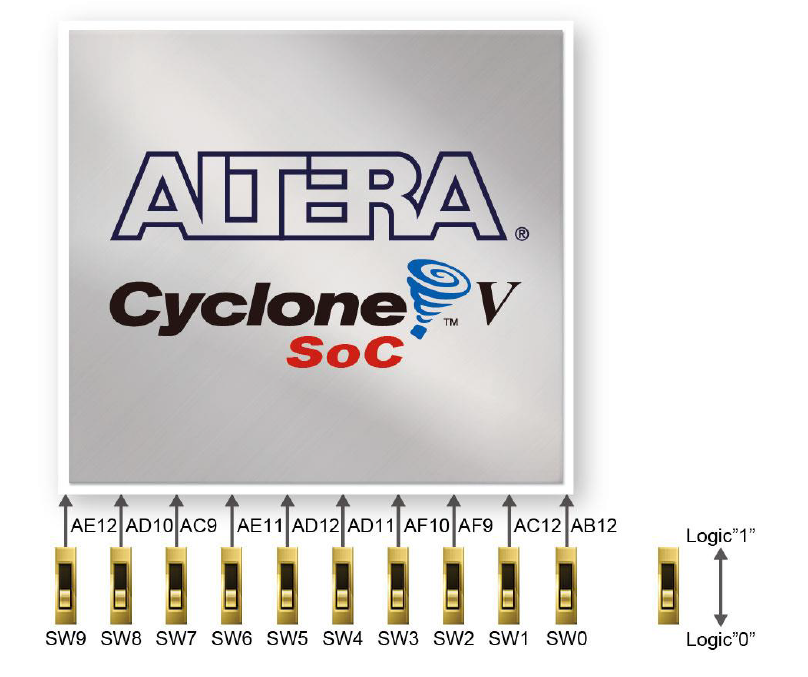
\includegraphics[width=0.47\textwidth]{switchbuttons}
		\caption{\label{fig:switchbuttons} Switch Buttons}
	\end{figure}
	
	
	
	\-\\[1cm]
	
	\section{Modules}
	\- \indent
	The modules and functional blocks designed and used in the project are presented in this section.
	%\begin{figure}[h!]
	%	\centering
	%	\begin{subfigure}{.48\textwidth}
	%		\centering
	%		\includegraphics[width=1\linewidth]{scope_28_SimResult}
	%\caption{Theoretical Output of VCO.}
	%\label{fig:VCOFor1kHzTheoretical}
	%	\end{subfigure}%
	%	\newline
	%	\begin{subfigure}{.48\textwidth}
	%		\centering
	%		\includegraphics[width=1\linewidth]{scope_28}
	%\caption{Practical Output of VCO.}
	%\label{fig:VCOFor1kHzPractical}
	%	\end{subfigure}
	%\caption{VCO Outputs for 1kHz.}
	%	\label{fig:VCOFor1kHz}
	%\end{figure}
	
	\subsection{ADC} \- \indent
	This module quantizes the analog input data. The hardware used is LTC2308 that is built into the FPGA. The Altera provides an example code regarding the use of the built-in ADC\cite{b1}. By evaluating the provided functionalities of this example with the help of a MsC project \cite{b2}, a code is written in Verilog HDL and in Qsys environment. Qsys instantiates the internal connections of embedded modules to use ADC controller. The resulting Qsys module is exported as BSF file and that is shown in \textit{Figure~\ref{fig:adc_block}}.
	
	This module couldn't be used in the project since the VGA screen wasn't driven. It wasn't possible to test the output of the ADC module. Also, integration of the module with the rest of the project couldn't be done.
	
	\begin{figure}[H]
		\setlength{\unitlength}{\textwidth}
		\center 
		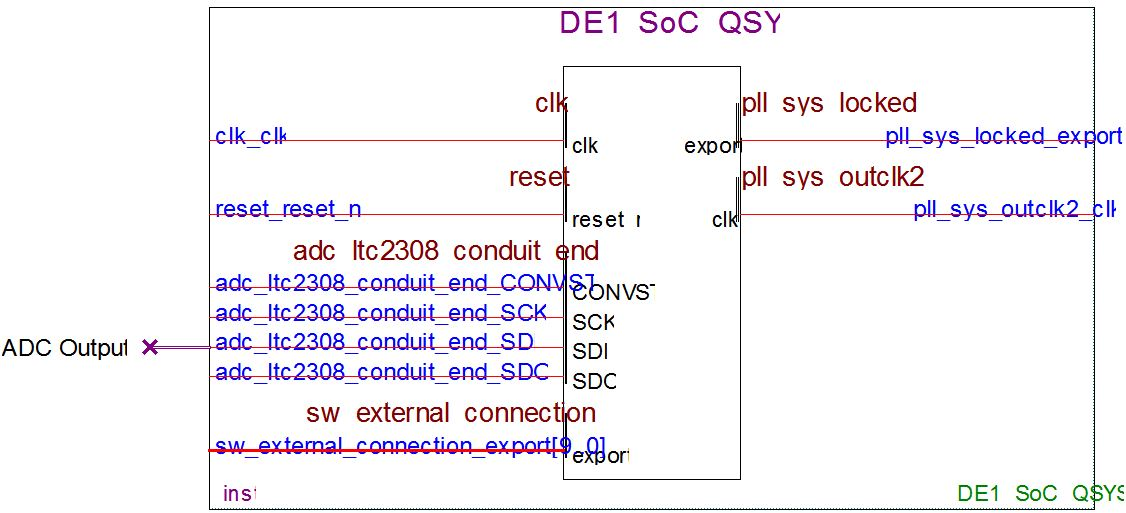
\includegraphics[width=0.47\textwidth]{adc_block}
		\caption{\label{fig:adc_block}The Block Diagram of the ADC}
	\end{figure}
	
	\subsection{RAM} \- \indent
	The main function of RAM is to introduce a block to the system that can be both writable and readable. Writing is necessary to save data coming from ADC and reading is also necessary to process the data and show them on VGA screen. The RAM should work with FIFO structure to realize proper operation on VGA screen. "A FIFO (first-in-first-out) buffer is an "elastic" storage between two subsystems."\cite{b3}. A FIFO based read and write operation is depicted in \textit{Figure~\ref{fig:fifo_diagram}}. The FIFO is designed and written, the resulting circuit block is shown in \textit{Figure~\ref{fig:fifo_diagram}}. The implemented FIFO has 8 bits of stack height and 12 bits of stack width. It also indicates when stacks are half-filled or full-filled.
	
	Throughout the project, the RAM unit functions as a memory of the system. Firstly, the data coming from the output of the ADC is written to the RAM and secondly, the necessary calculations are made by calculation unit and written the data again. Finally, with a proper frequency, the data is read by VGA controller in order to reflect the wanted signal to the monitor. If this part is not working properly, the overall project can not operate properly. 
	
	In the demo, this module wasn't shown due to incompleteness of the rest of the project, even though FIFO was working properly.
	
	\begin{figure}[t!]
		\setlength{\unitlength}{\textwidth}
		\center 
		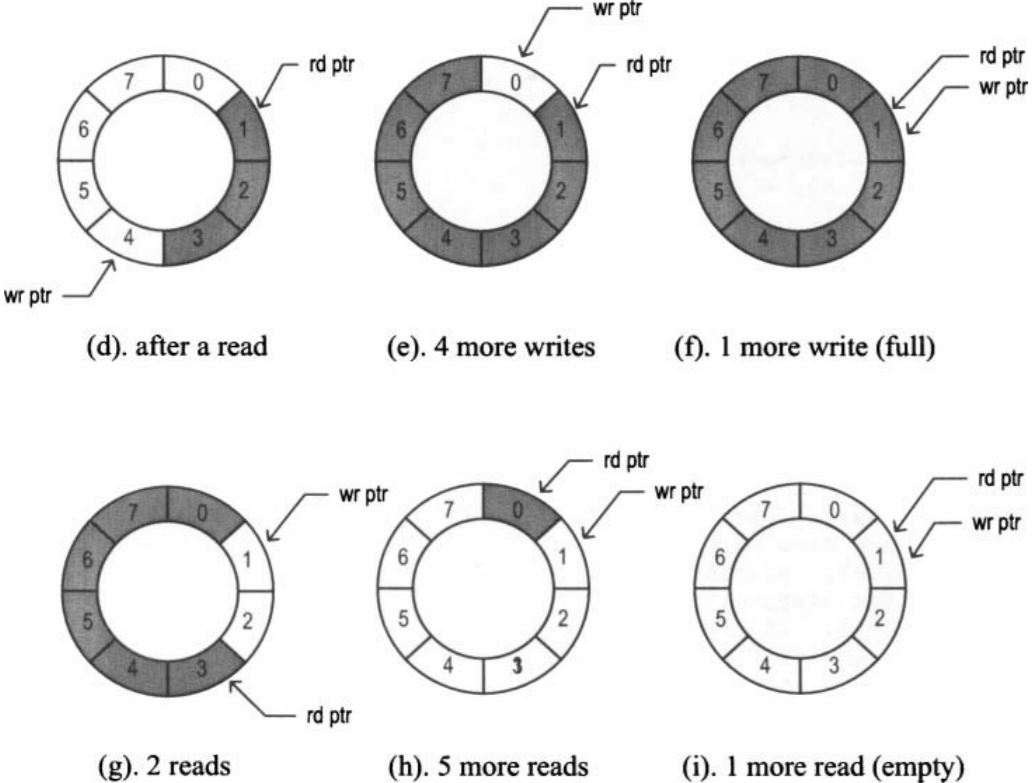
\includegraphics[width=0.47\textwidth]{fifo_diagram}
		\caption{\label{fig:fifo_diagram}FIFO Working Principle\cite{b3}}
	\end{figure}
	
	\begin{figure}[h!]
		\setlength{\unitlength}{\textwidth}
		\center 
		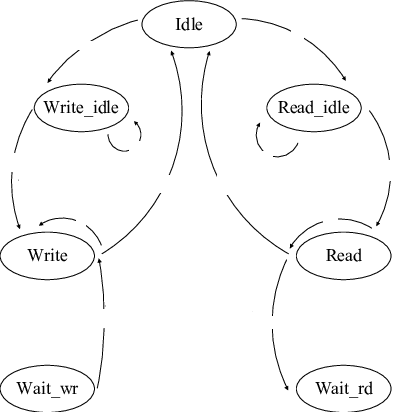
\includegraphics[width=0.47\textwidth]{RAM_state}
		\caption{\label{fig:RAM State} State Diagram for RAM}
	\end{figure}
	
	\begin{figure}[h!]
		\setlength{\unitlength}{\textwidth}
		\center 
		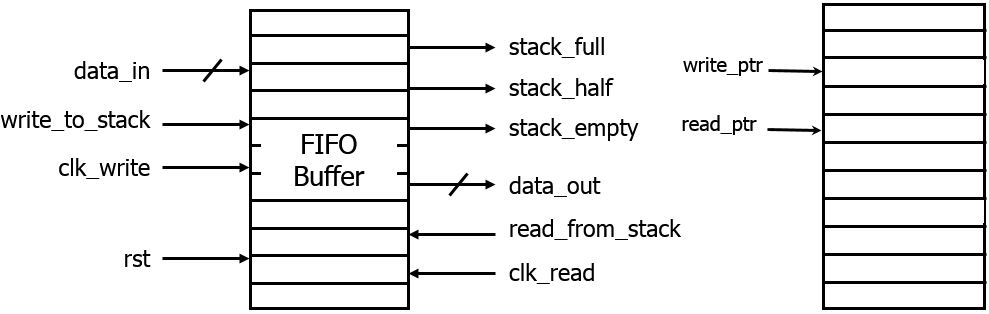
\includegraphics[width=0.47\textwidth]{fifo_ports}
		\caption{\label{fig:fifo_ports} FIFO Block}
	\end{figure}
	
	
	\subsection{Computation Unit} \- \indent
	Computation unit is the unit responsible for all kinds of mathematical calculation of the project. For instance mean value calculation for the input signal are conducted in this unit. This Unit can be considered as a brain of the project. Some important parts are as follows,	
	
	\begin{figure}[h!]
		\setlength{\unitlength}{\textwidth}
		\center 
		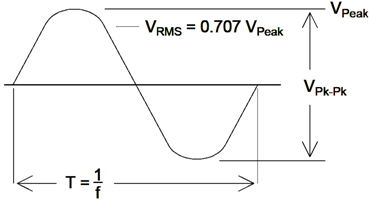
\includegraphics[width=0.47\textwidth]{voltage}
		\caption{\label{fig:waveform} Voltage Waveform and its Properties}
	\end{figure}
	
	
	
	\subsubsection{Calculation of Peak-to-Peak Value }	
	\- \indent
	To find the peak-to-peak value of the input voltage, we needed to find the maximum and minimum voltage values of the given input. For that purpose we have used a well known sorting algorithm. Initially a point on the waveform was picked and every point next to it was compared to it. If the next point on the voltage is bigger than the initially stored value, the stored value is replaced with that value. After tracing every point on the waveform, the biggest value can be found. Similarly, the lowest value on the voltage waveform can be found. 
	
	After finding minimum and maximum points at the voltage waveform, peak-to-peak value is the difference between these values as can be seen from the \textit{Figure~\ref{fig:waveform}}.  	
	
	
	\subsubsection{Calculation of Mean Value}
	
	
	\subsubsection{Calculation of DC Offset}
	
	DC offset is a mean amplitude displacement from
	
	
	\subsubsection{Calculation of Frequency}
	
	
	
	\subsubsection{Mode Selection (AC/DC)} \- \indent
	AC/DC Modes are one of the most fundamental mods of digital oscilloscopes in market. In this part we will build a module to build our own selection mode. One slide switch will be assigned to retrieve the desired mode information from the user. Based on this information, screen will display the input signal either with the DC offset or without the DC offset.
	
	\subsubsection*{AC Mode} \- \indent
	In AC Mode operation of the oscilloscope, the DC offset voltage is removed from the input voltage before it is reflected to the VGA monitor. For that the DC offset data found earlier will be removed from stored data.
	
	\subsubsection*{DC Mode} \- \indent
	In DC Mode operation of the oscilloscope, the DC offset voltage is untouched from the stored data of the input voltage. The stored data is reflected directly to the VGA monitor. 
	
	
	\subsection{VGA Screen} \- \indent
	VGA is a widely used standard in video industry for the transmission of video signals from a computer or microprocessor into a monitor or TV. The input pin configuration for the VGA Monitor can be seen at \textit{Figure~\ref{fig:vga_pins}}. VGA provides 640x480 pixel resolution. This resolution, however, is not the total pixel in horizontal and vertical axes. There is a blank border frame surrounding the display area. The horizontal axis has 48 pixels of border width on the left and 16 pixels of border width on the right side of the screen. Additionally, there are 96 pixels of border width for ray tube the retrace through the diagonal of the screen. The vertical axis has also similar additional pixels. 10 and 33 pixels for top and bottom borders, respectively. Also 2 pixels for the vertical retrace of the ray tube. The total structure of a VGA screen can be seen in \textit{Figure~\ref{fig:vga-hsync-vsync}}. The whole screen is 800x525 pixels.
	
	\begin{figure}[h!]
		\setlength{\unitlength}{\textwidth}
		\center 
		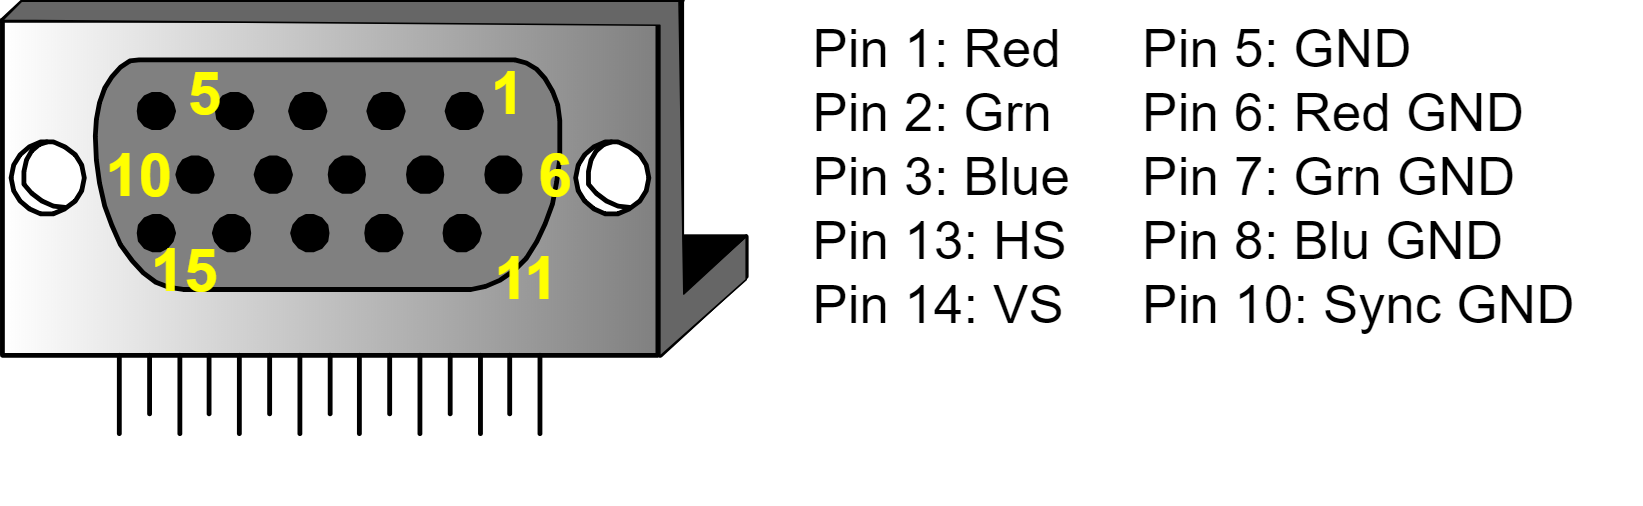
\includegraphics[width=0.47\textwidth]{vgapins}
		\caption{\label{fig:vga_pins} VGA Input Pins}
	\end{figure}
	
	
	\begin{figure}[h!]
		\setlength{\unitlength}{\textwidth}
		\center 
		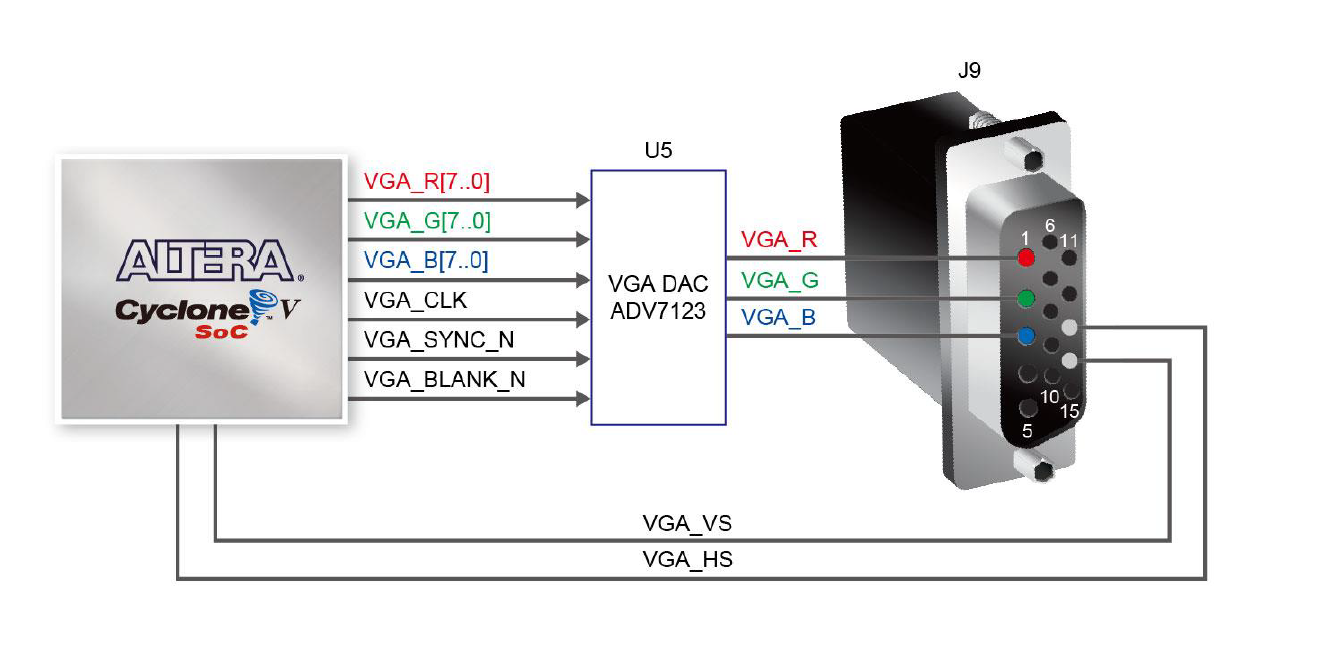
\includegraphics[width=0.47\textwidth]{VGAconfig}
		\caption{\label{fig:VGA_config}The Block Diagram of the Project}
	\end{figure}
	
	\begin{figure}[h!]
		\setlength{\unitlength}{\textwidth}
		\center 
		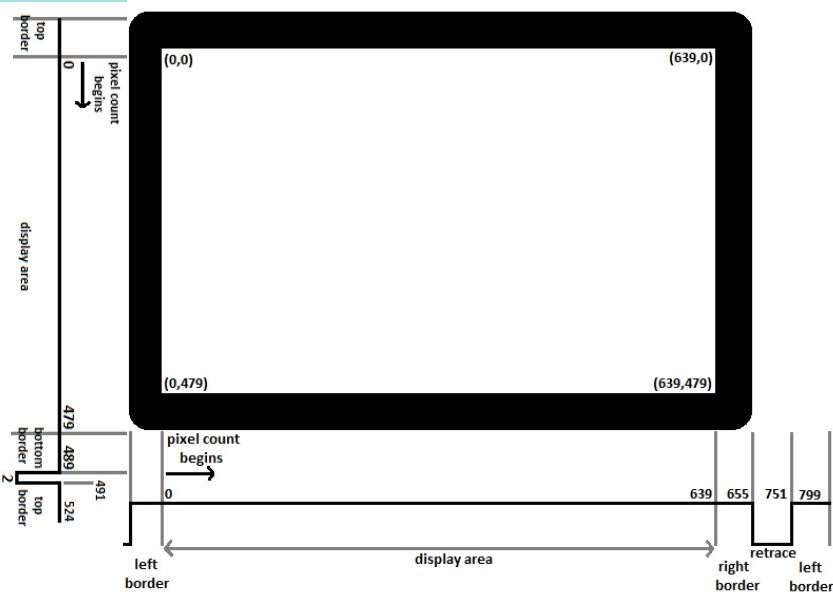
\includegraphics[width=0.47\textwidth]{vga-hsync-vsync}
		\caption{\label{fig:vga-hsync-vsync}A Frame of VGA Screen with Control Signals}
	\end{figure}
	
	\subsubsection{VGA Controller} \- \indent
	
	The VGA controller administrates the digitally stored input signal and the measured properties of the signal to display them on the screen. The two counters in this module, named "h\_count" and "v\_count" are to keep track of the vertical and horizontal pixels. Also there are two more counters to synchronize the display area, blank are and the retrace area of the screen. These counters are "h\_sync" and "v\_sync" and they are the output signals of PINs 13 and 14 of VGA output with an active low behaviour. Lastly, "o\_red", "o\_blue" and "o\_green" are the 8-bit output bus signals determine the color of the respective pixel by mapping them on 255,255,255 color scale. The resulting diagram showing the signals of the VGA Controller is shown in  \textit{Figure~\ref{fig:vgacontroller}} \cite{b4}.
	
	The waveform, frequency, peak-to-peak voltages of the signals are dynamic measurements, while texts indicating them are not. For this reason, with the reference of \cite{b2}, static images can be shown in ".MIF" formats for simplicity. These images are first saved as ".BMP" then converted to ".MIF" and stored in a simple ROM structure.
	
	The codes are written alongside with the aforementioned ideas, however, the display on the VGA screen could not be achieved. 
	
	combines the data from RAM and Computation Unit to create a signal that can be displayed on the VGA monitor. Each of the RAM Modules contains an image that is ready for display on the screen. However, the data must be positioned relative to each other and combined. Also this module performs once a second as desired in the project requirements. The VGA controller also gets data from different data inputs such as Time/div and Voltage/div in order to reflect the waveform as user requires. In this part multiple clock signals and counters needed to display the waveform accordingly. Basic VGA Controller can be seen at \textit{Figure~\ref{fig:vga_controller}}.
	
	\begin{figure}[h!]
		\setlength{\unitlength}{\textwidth}
		\center 
		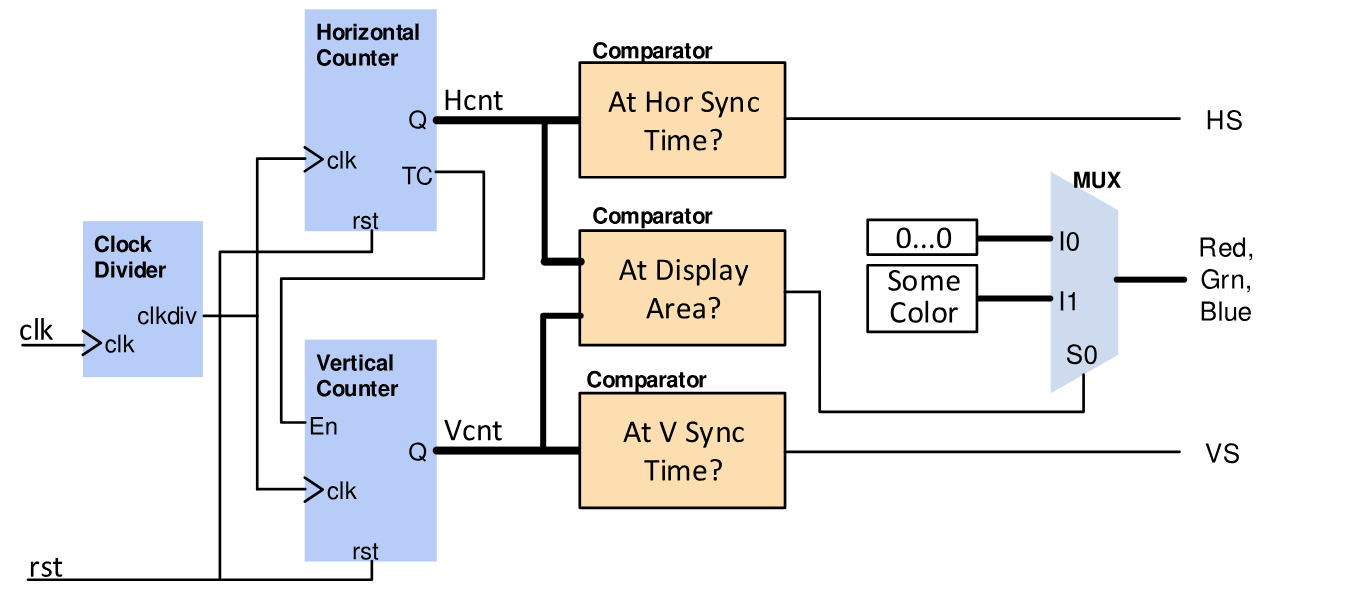
\includegraphics[width=0.47\textwidth]{vgacontroller}
		\caption{\label{fig:vgacontroller} Internal Structure of the VGA Controller}
	\end{figure}
	
	
	\section{Conclusion}
	\- \indent
	In this project, the aim was to design a FPGA based digital oscilloscope using Verilog. The project consisted of four main part that are Analog to Digital Converter, RAM, Computation Unit and VGA Screen. Overall diagram of the project can be seen at \textit{Figure~\ref{fig:overall_diagram}}. None of the parts were implemented properly. This is due to lack of knowledge in Verilog, RAM structure, internal flow of data in FPGA and computer structure. It would be better to implement some parts of the project as the project but the project itself was too complex to build for us. The importance of Verilog is understood very well.
	
	
	
	\begin{thebibliography}{00}
		\bibitem{b1} “De1-Soc CD.” [Online]. Available: http://download.terasic.com/downloads/cd-rom/de1-soc/DE1-SoC\_v.5.0.1\_HWrevF\_SystemCD.zip. [Accessed: 21-May-2018].
		\bibitem{b2} “Digital Scope Implemented on Altera DE1-SoC.” [Online]. Available: https://people.ece.cornell.edu/land/courses/eceprojectsland/STUDENTPROJ/\\2015to2016/hj424/hj424\_report\_201605191237.pdf. [Accessed: 21-May-2018].
		\bibitem{b3} P.P. Chu, Embedded SoPC Design with NIOS II Processor and Verilog Examples. New Jersey, 2012.
		%\bibitem{b3} “2N7000 Datasheet.” [Online]. Available: https://www.onsemi.com/pub/Collateral/2N7000-D.PDF. [Accessed: 20-Jan-2018].
		\bibitem{b4} "VGA Display Controller" [Online]. Avaible : https://learn.digilentinc.com/Documents/269
		%\bibitem{b6} Y. Yorozu, M. Hirano, K. Oka, and Y. Tagawa, ``Electron spectroscopy studies on magneto-optical media and plastic substrate interface,'' IEEE Transl. J. Magn. Japan, vol. 2, pp. 740--741, August 1987 [Digests 9th Annual Conf. Magnetics Japan, p. 301, 1982].
		%\bibitem{b7} M. Young, The Technical Writer's Handbook. Mill Valley, CA: University Science, 1989.
	\end{thebibliography}
	
	
	
	
\end{document}
